\section{Resultados y validación}

\subsection{Resultados experimentales}

Los resultados experimentales confirman que la separación entre detección y clasificación es adecuada. El detector YOLO26n localiza grupos solares y genera recortes para la etapa morfológica.\citep{ultralyticsYOLO26,mcintosh1990classification,palladino2022sunspot}.

El clasificador jerárquico conserva salidas separadas para $Z$, $P$ y $C$, con un F1 promedio cercano a los mejores valores de referencia considerados. Esta decisión evita compactar artificialmente clases raras y ofrece al usuario probabilidades y alternativas plausibles, en lugar de una única etiqueta opaca \citep{sayez2023sunscc,deng2025mcintosh,woo2023convnextv2}.

\begin{figure}[H]
    \centering
    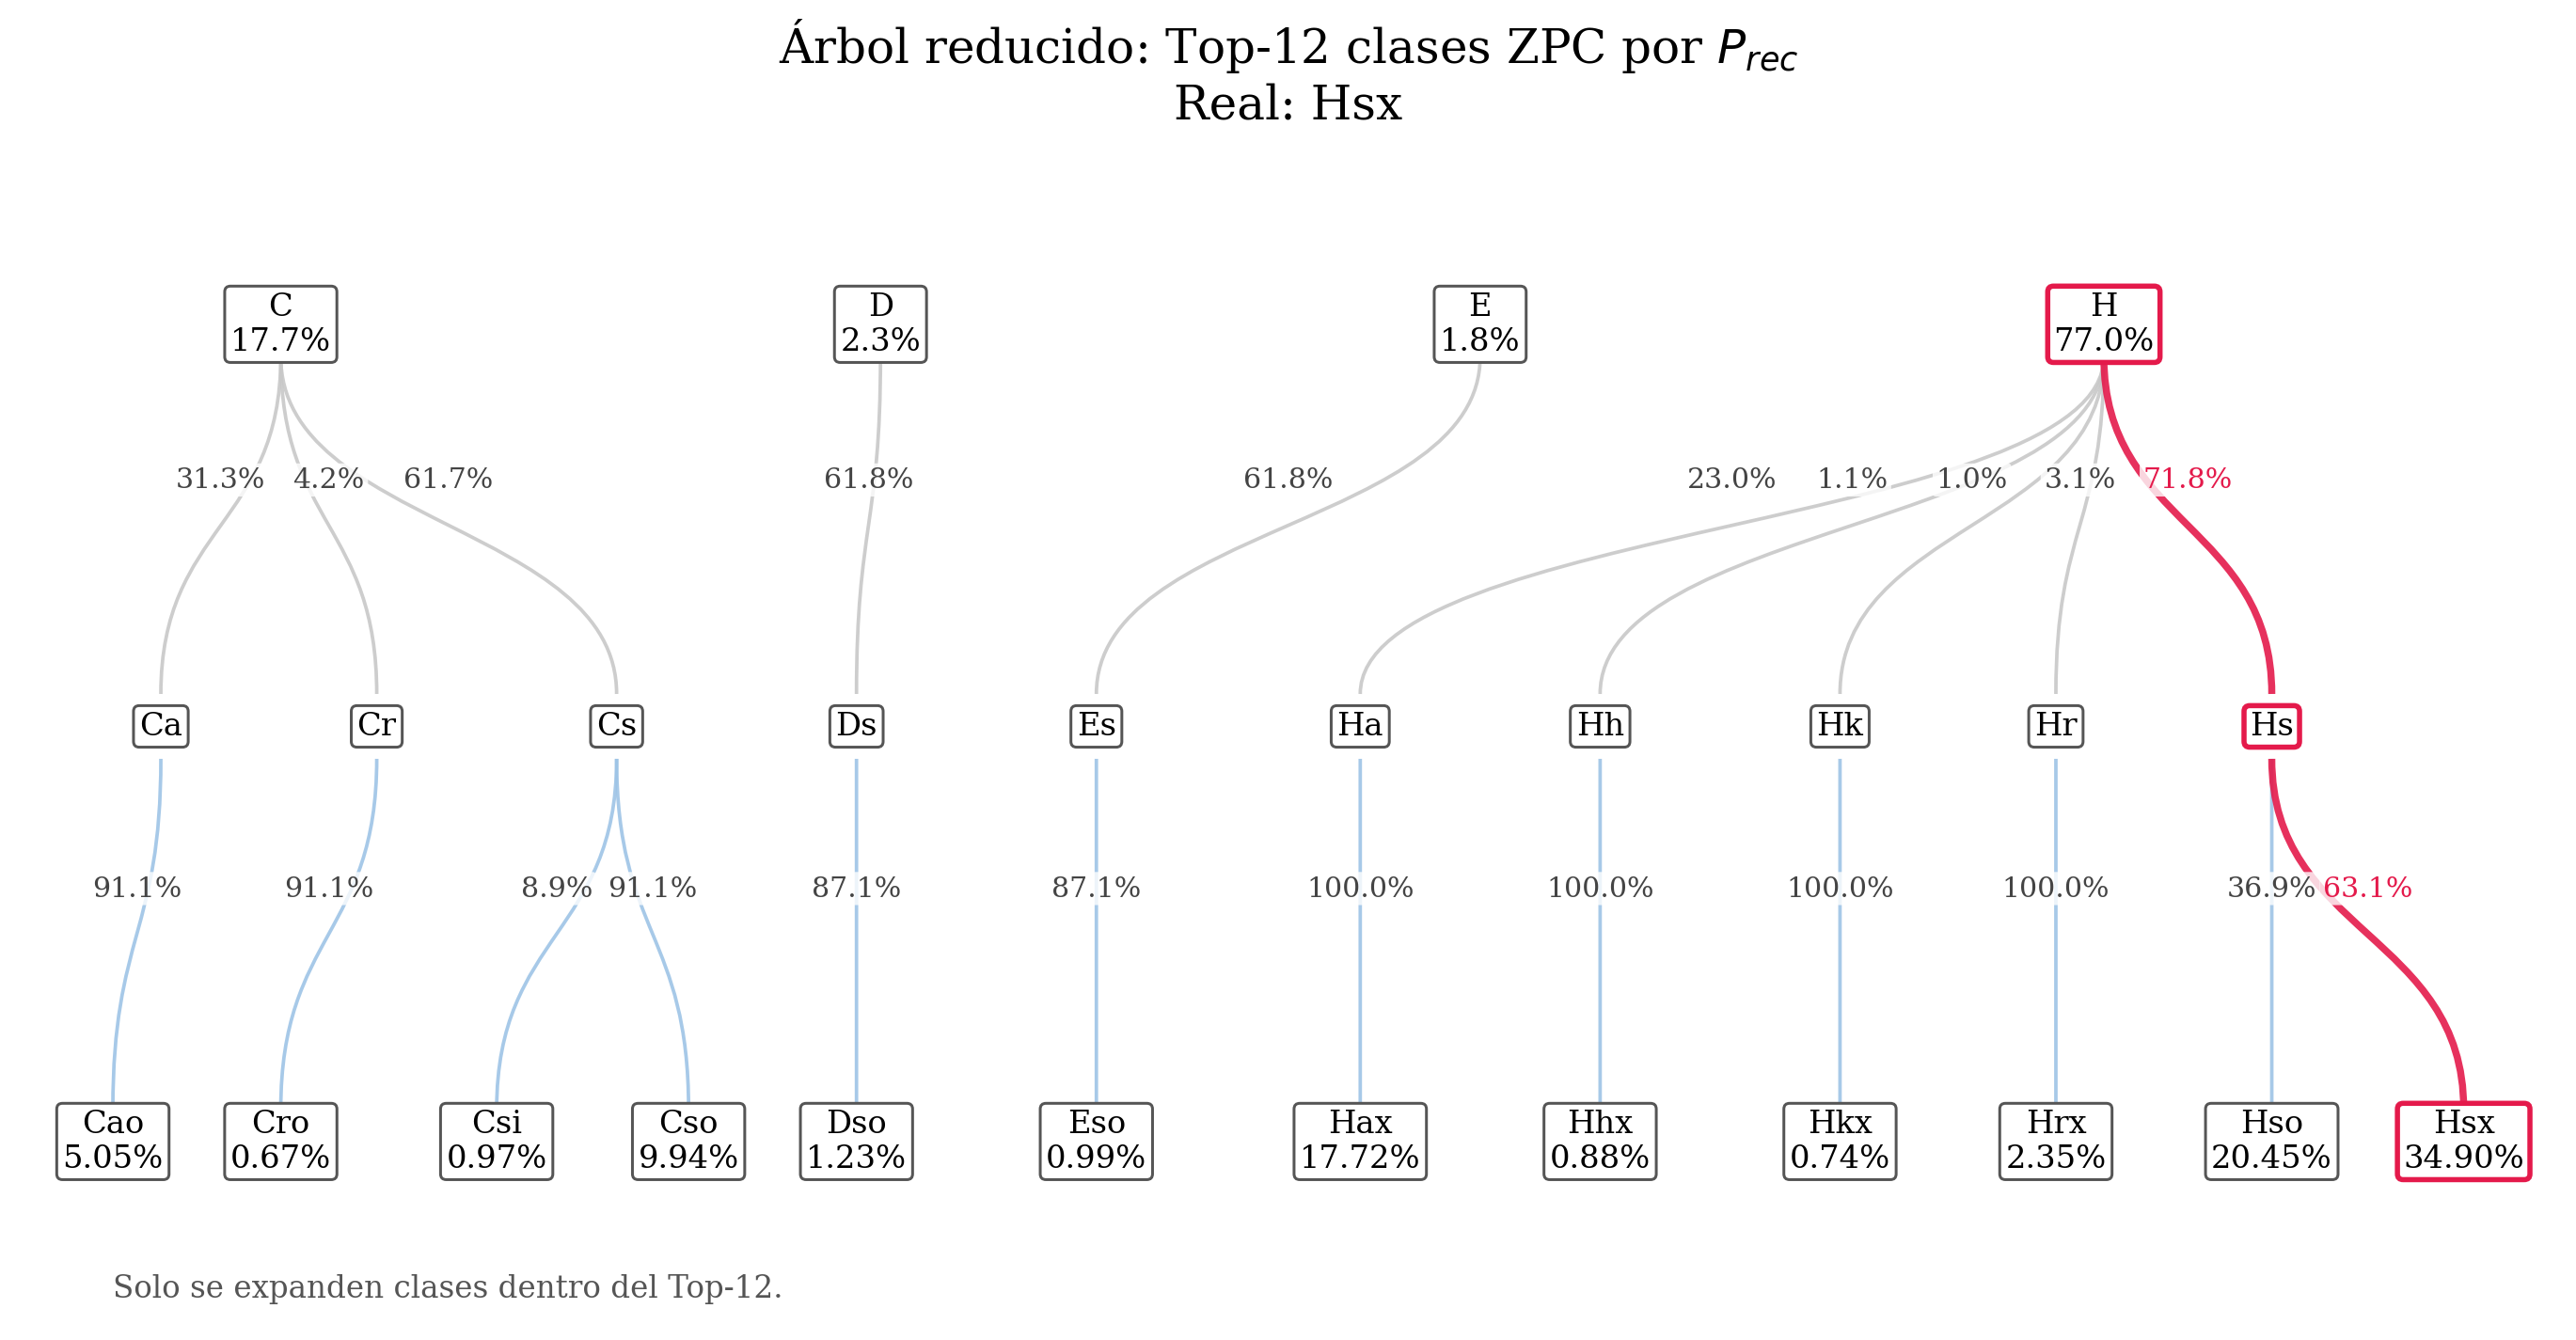
\includegraphics[width=0.92\linewidth]{figures/ml/top12_tree.png}
    \caption{Árbol bayesiano de probabilidades para la recomendación jerárquica Zurich--McIntosh. La visualización organiza alternativas probables según $Z$, $P$ y $C$, preservando consistencia taxonómica. \textbf{Fuente:} Elaboración propia.}
    \label{fig:resumen-arbol-probabilidades}
\end{figure}

El árbol de probabilidades implementa la distribución $P_{\mathrm{rec}}(Z,P,C\mid x)$ definida en el diseño del software. Esta representación permite inspeccionar cómo se reparte la confianza desde el tipo de grupo hacia las componentes penumbrales y de compactación, lo que resulta útil cuando varias configuraciones morfológicas son cercanas \citep{mcintosh1990classification,bornmann1994flarerates}.

\begin{figure}[H]
    \centering
    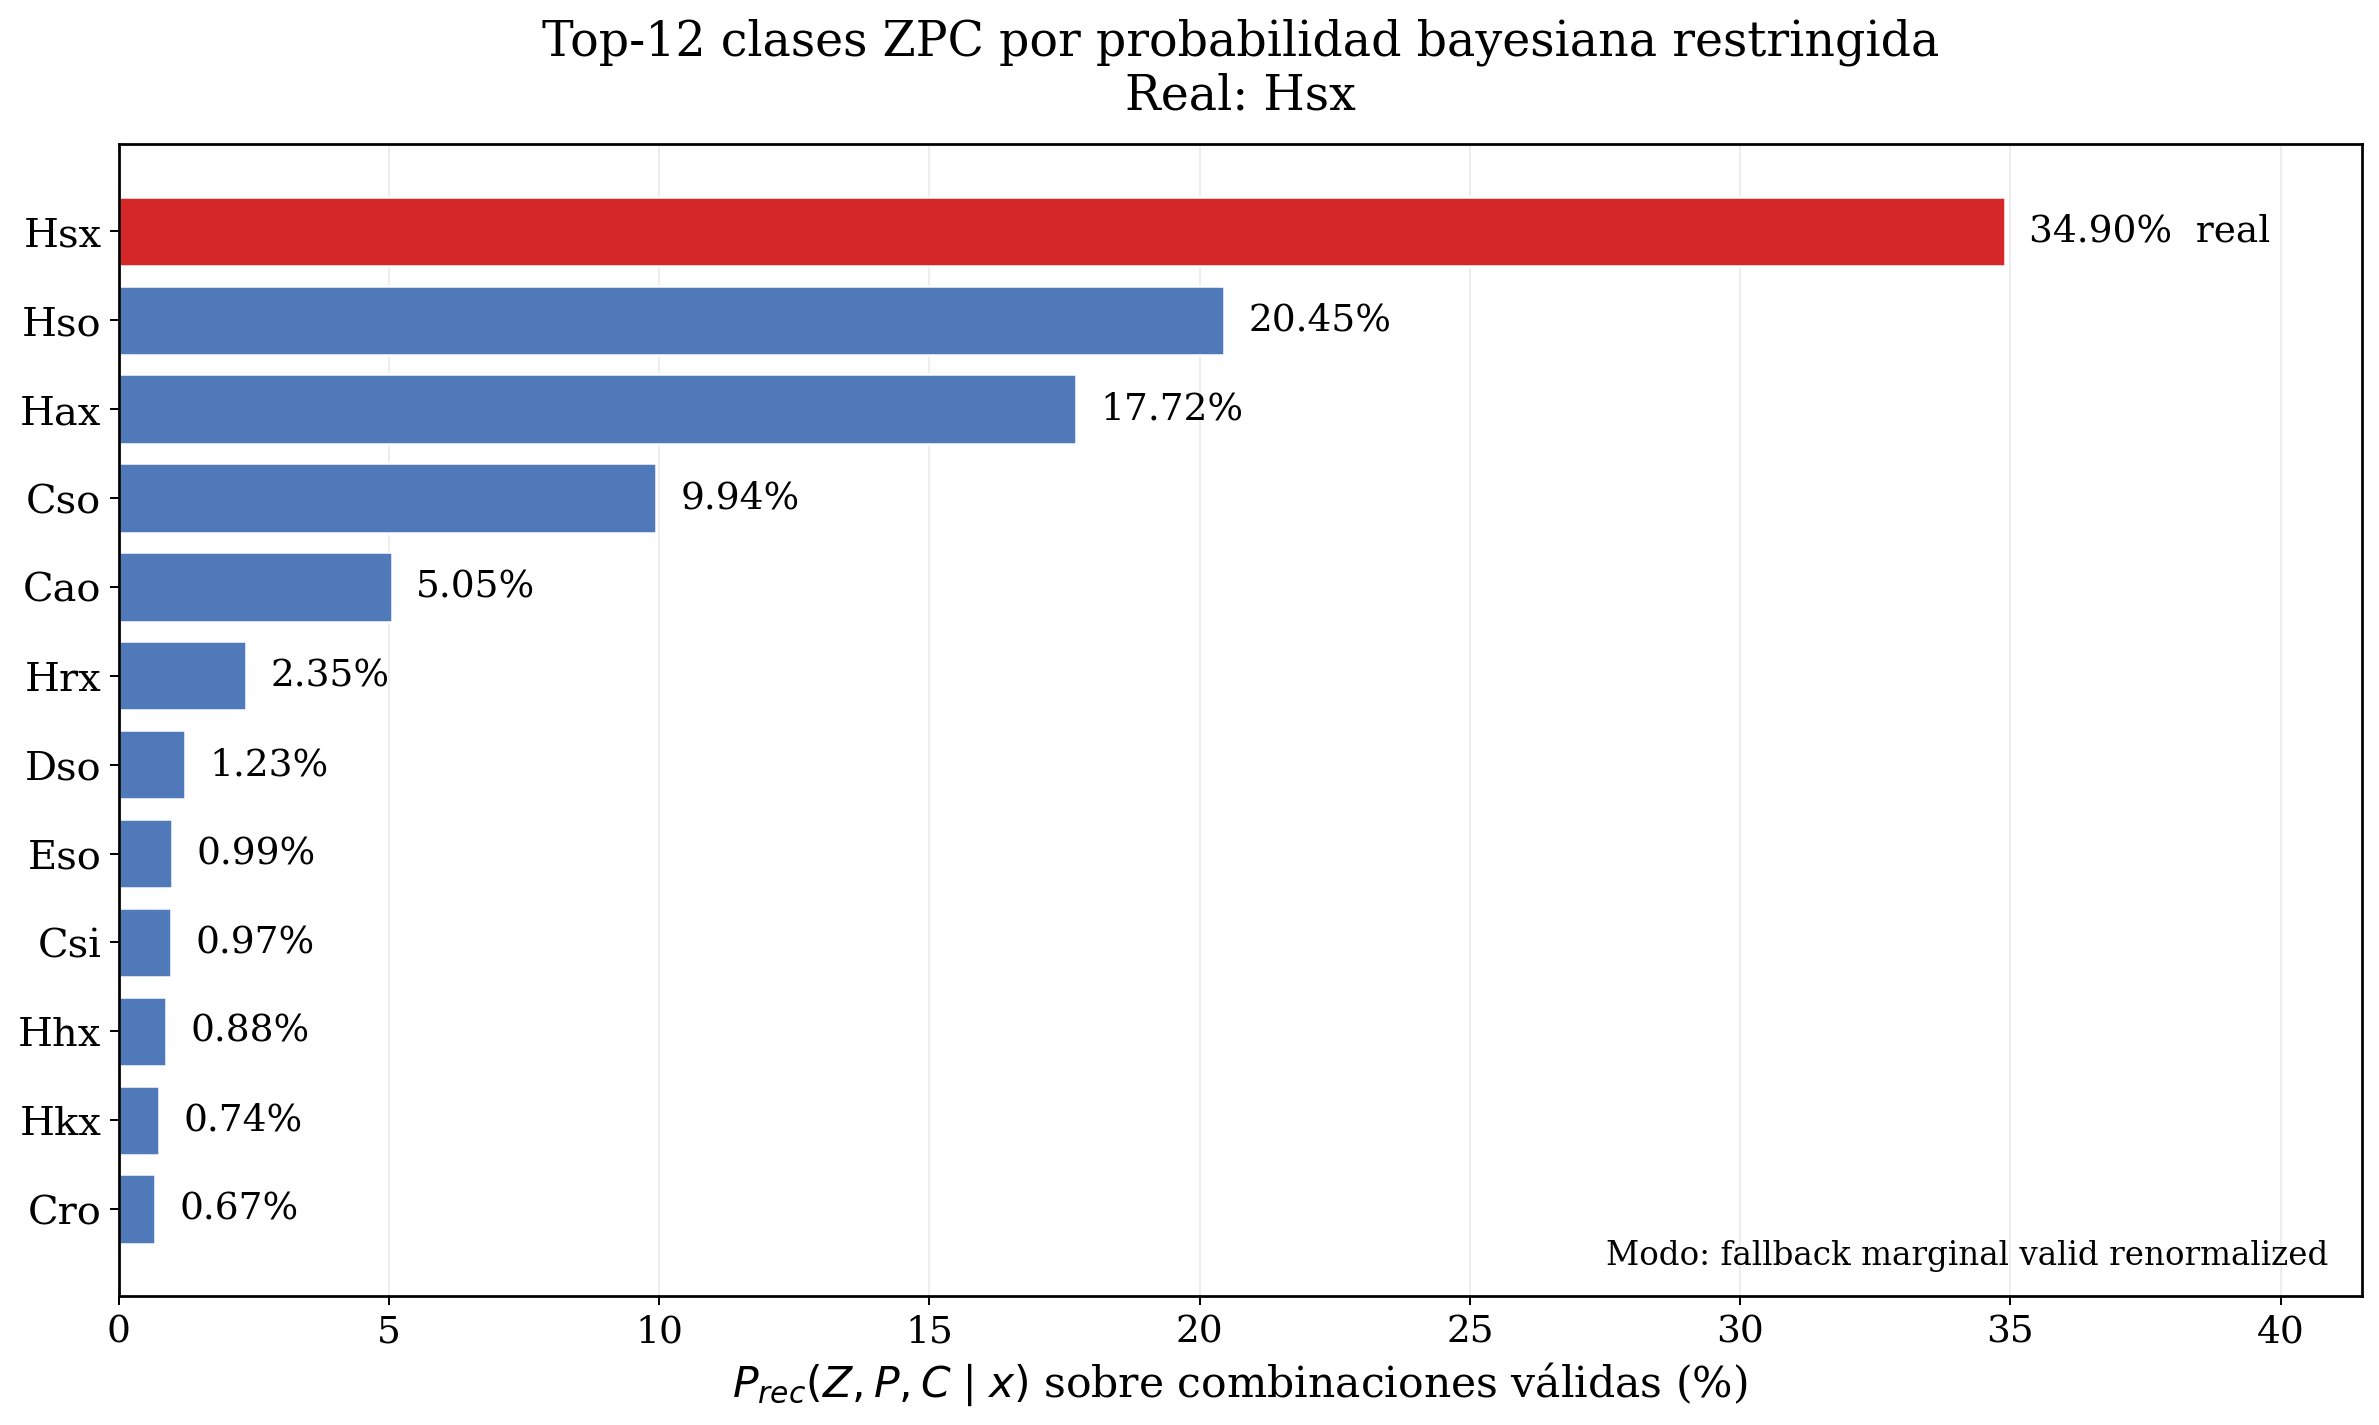
\includegraphics[width=0.92\linewidth]{figures/ml/top12_rec.png}
    \caption{Histograma de las doce clases Zurich--McIntosh con mayor probabilidad bayesiana restringida. \textbf{Fuente:} Elaboración propia.}
    \label{fig:resumen-top12-probabilidades}
\end{figure}

\begin{table}[H]
\centering
\caption{Comparación resumida de F1 por componente Zurich--McIntosh. \textbf{Fuente:} Elaboración propia a partir de los resultados del libro.}
\label{tab:resumen-f1}
%\scriptsize
\begin{tabular}{lcccc}
\toprule
\textbf{Modelo} & \textbf{$Z$} & \textbf{$P$} & \textbf{$C$} & \textbf{Prom.} \\
\midrule
Palladino et al. & 0.65 & 0.54 & 0.84 & 0.68 \\
Deng et al. & 0.47 & 0.41 & 0.60 & 0.49 \\
Propuesta & 0.65 & 0.63 & 0.71 & 0.66 \\
\bottomrule
\end{tabular}
\end{table}

Las métricas por clase permiten identificar cuáles componentes de la taxonomía presentan mayor ambigüedad. Para cada clase $c$, se emplean precisión, \textit{recall} y F1, definidos a partir de verdaderos positivos, falsos positivos y falsos negativos; esta lectura es necesaria porque el conjunto presenta desbalance y clases morfológicamente cercanas \citep{mcintosh1990classification,cui2019classbalanced,sayez2023sunscc}.

\begin{table}[H]
\centering
\caption{Métricas para salida $Z$. \textbf{Fuente:} Elaboración propia.}
\label{tab:resumen-metricas-z}
%\scriptsize
\begin{tabular}{lccc}
\toprule
\textbf{Clase} & \textbf{Precisión} & \textbf{Recall} & \textbf{F1} \\
\midrule
A & 0.79 & 0.73 & 0.76 \\
B & 0.74 & 0.71 & 0.72 \\
C & 0.68 & 0.61 & 0.64 \\
D & 0.63 & 0.61 & 0.62 \\
E & 0.49 & 0.39 & 0.43 \\
F & 0.47 & 0.39 & 0.43 \\
H & 0.78 & 0.84 & 0.81 \\
Prom. pond. & 0.68 & 0.63 & 0.65 \\
\bottomrule
\end{tabular}
\end{table}


\begin{table}[H]
\centering
\caption{Métricas para salida $P$. \textbf{Fuente:} Elaboración propia.}
\label{tab:resumen-metricas-p}
%\scriptsize
\begin{tabular}{lccc}
\toprule
\textbf{Clase} & \textbf{Precisión} & \textbf{Recall} & \textbf{F1} \\
\midrule
x & 0.57 & 0.31 & 0.40 \\
r & 0.34 & 0.28 & 0.31 \\
s & 0.59 & 0.63 & 0.61 \\
a & 0.46 & 0.54 & 0.50 \\
h & 0.71 & 0.65 & 0.68 \\
k & 0.84 & 0.82 & 0.83 \\
Prom. pond. & 0.66 & 0.61 & 0.63 \\
\bottomrule
\end{tabular}
\end{table}


\begin{table}[H]
\centering
\caption{Métricas para salida $C$. \textbf{Fuente:} Elaboración propia.}
\label{tab:resumen-metricas-c}
%\scriptsize
\begin{tabular}{lccc}
\toprule
\textbf{Clase} & \textbf{Precisión} & \textbf{Recall} & \textbf{F1} \\
\midrule
x & 0.62 & 0.52 & 0.57 \\
o & 0.46 & 0.47 & 0.46 \\
i & 0.79 & 0.72 & 0.75 \\
c & 0.82 & 0.84 & 0.83 \\
Prom. pond. & 0.74 & 0.69 & 0.71 \\
\bottomrule
\end{tabular}
\end{table}

Los modelos predictivos se evaluaron con métricas escalares y espacio-temporales. Para el SSN, el error absoluto medio ($\mathrm{MAE}$) mide el promedio de las desviaciones absolutas entre los valores reales y las estimaciones. La calidad del ajuste escalar también se resume mediante el coeficiente de determinación ($R^2$), el cual evalúa la proporción de la varianza explicada por el modelo respecto al promedio de la serie observada $\bar{z}$. 

Para la reconstrucción latitudinal se emplea el error relativo de Frobenius ($E_F$), diseñado para cuantificar la fidelidad global de la matriz reconstruida. Además, la coherencia espacio-temporal se mide con la correlación ($\rho_{ST}$) entre las matrices vec-transformadas, y el desvío medio del centro latitudinal se define a través del error de latitud central ($\mathrm{MLCE}$). Estas métricas distinguen entre precisión escalar y fidelidad de la migración latitudinal \citep{kalman1960newapproach,schmid2010dmd,kutz2016dmd}.

\begin{figure}[H]
    \centering
    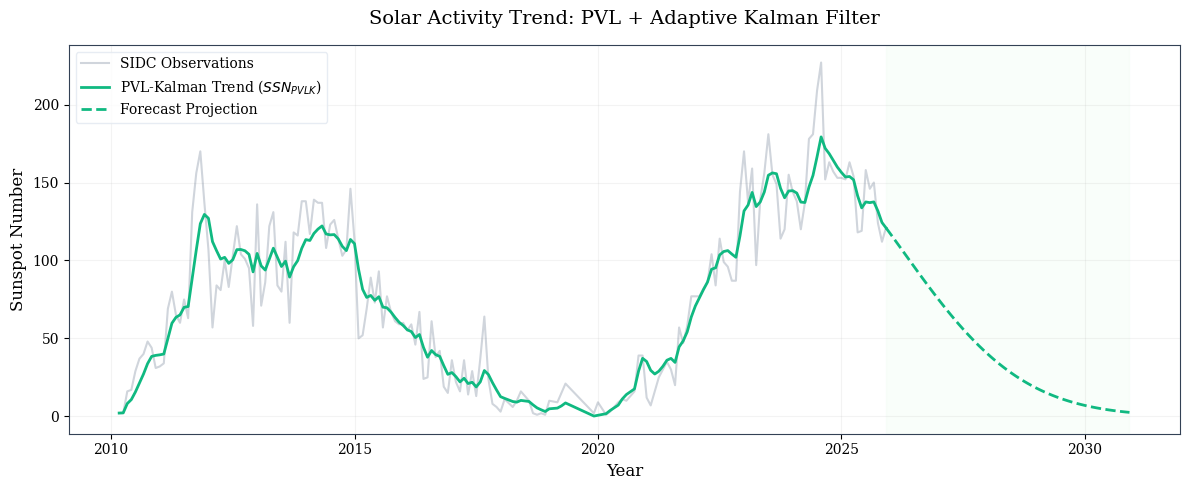
\includegraphics[width=0.92\linewidth]{figures/pred/kalman.png}
    \caption{Ajuste y predicción del número de manchas solares mediante PVL--Kalman. \textbf{Fuente:} Elaboración propia con base en el modelo PVL y el filtro de Kalman.}
    \label{fig:resumen-pvl-kalman}
\end{figure}

\begin{figure}[H]
    \centering
    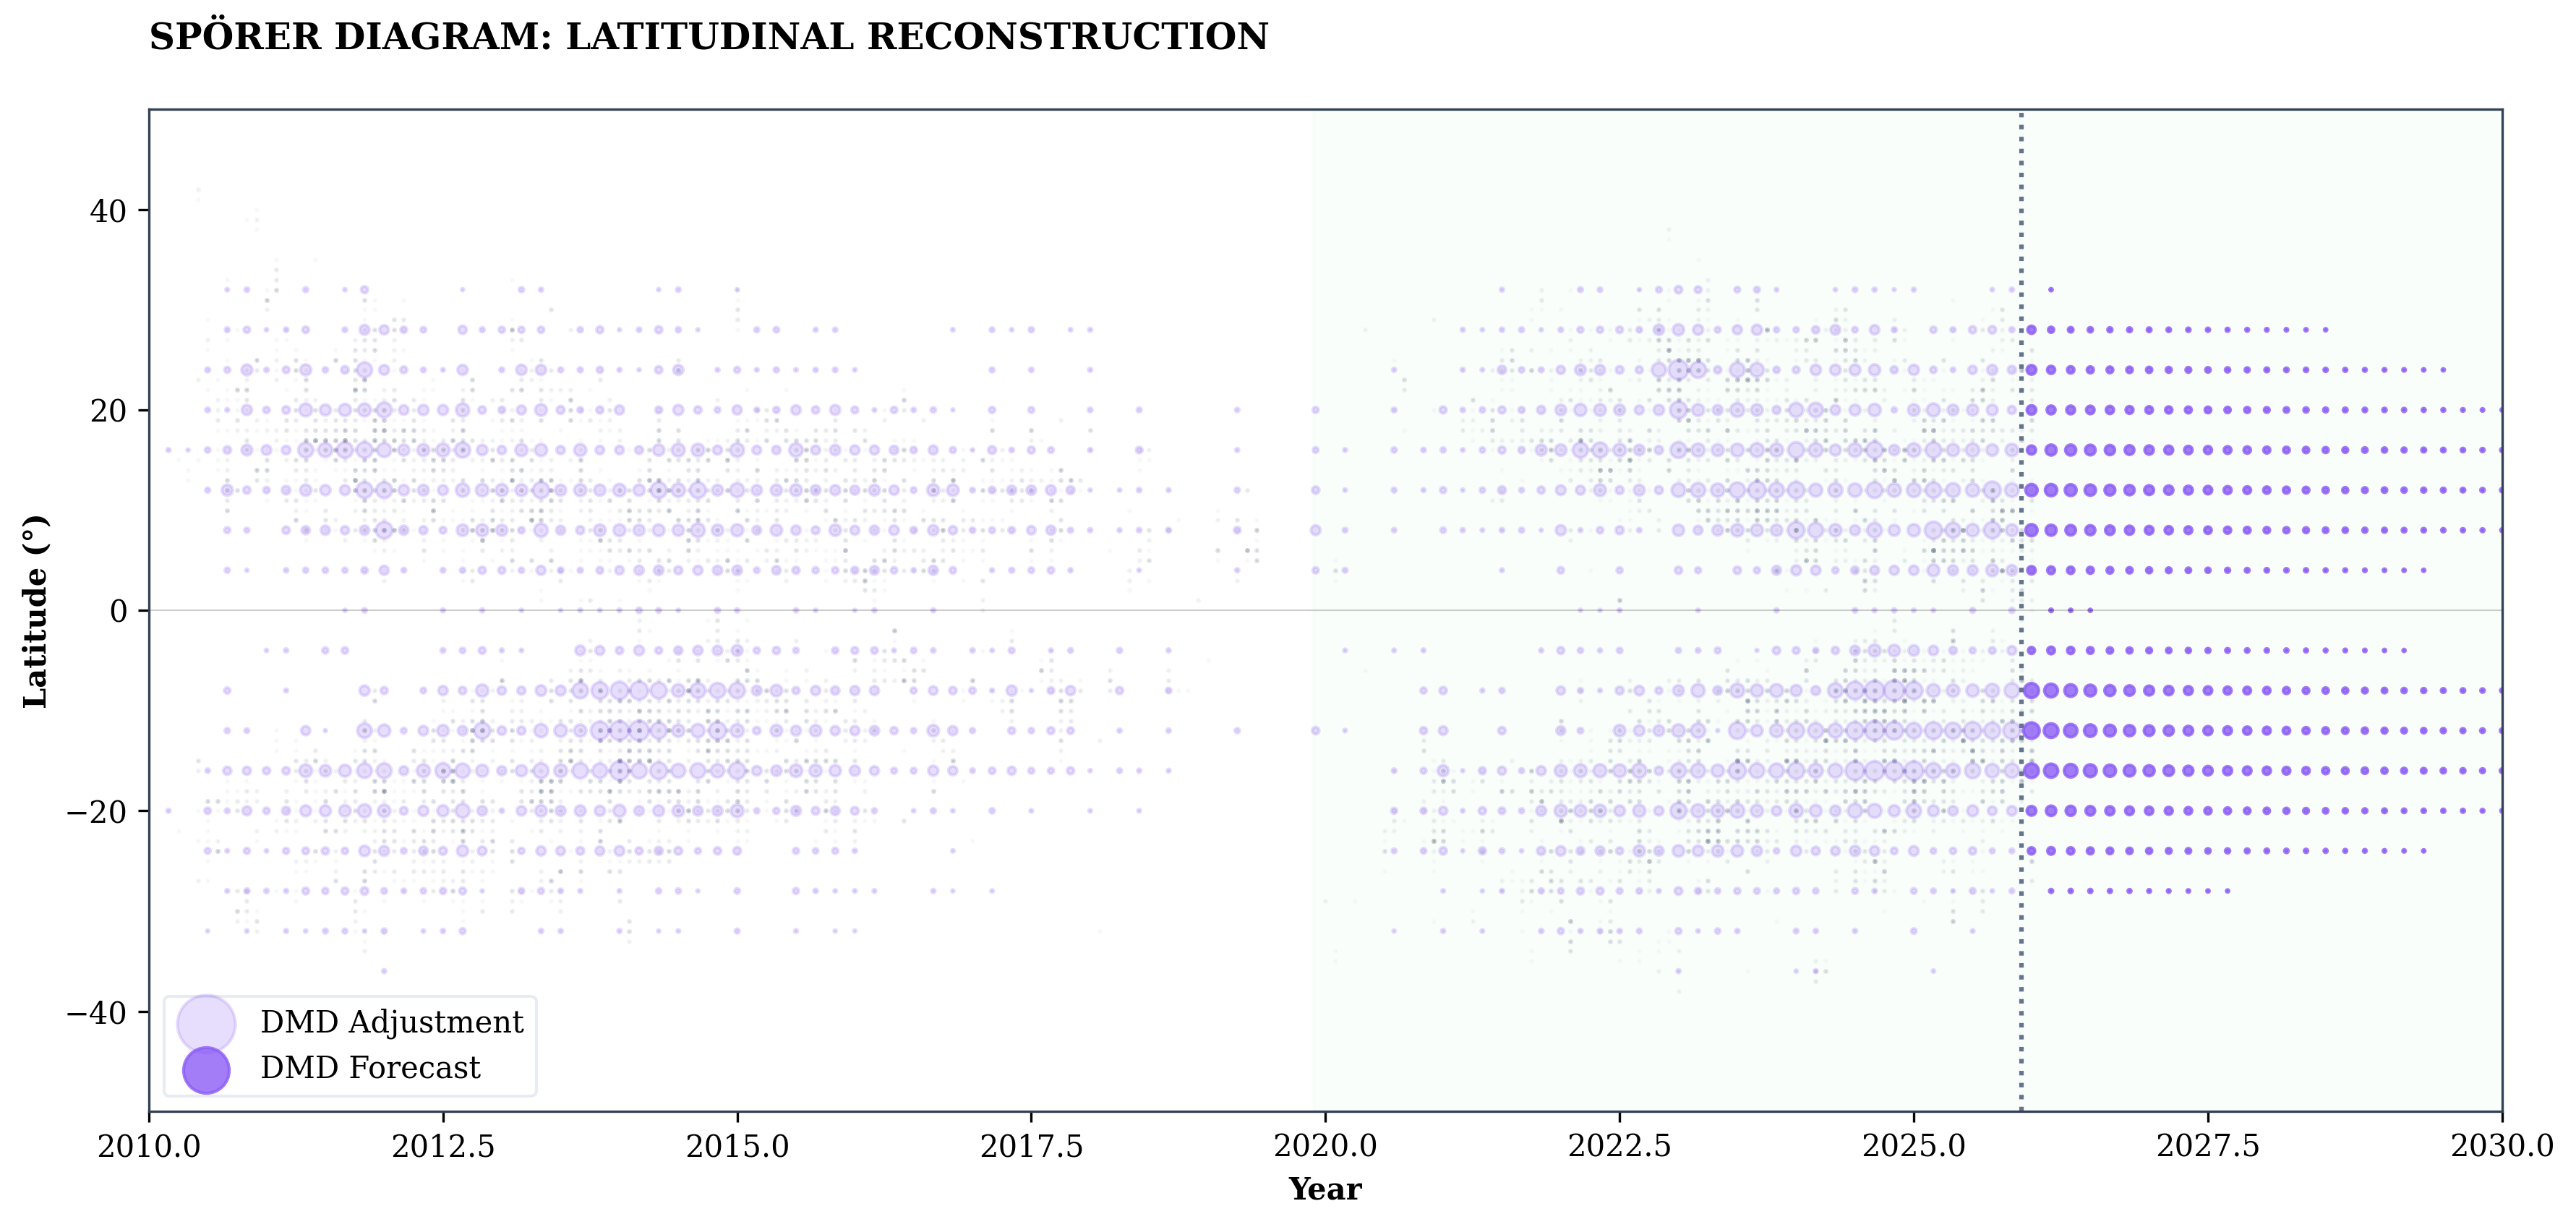
\includegraphics[width=0.92\linewidth]{figures/pred/sporer.png}
    \caption{Reconstrucción y predicción de la migración latitudinal de la actividad solar mediante DMD. La visualización conserva el patrón tipo diagrama de Spörer. \textbf{Fuente:} Elaboración propia.}
    \label{fig:resumen-sporer-dmd}
\end{figure}

\begin{figure}[H]
    \centering
    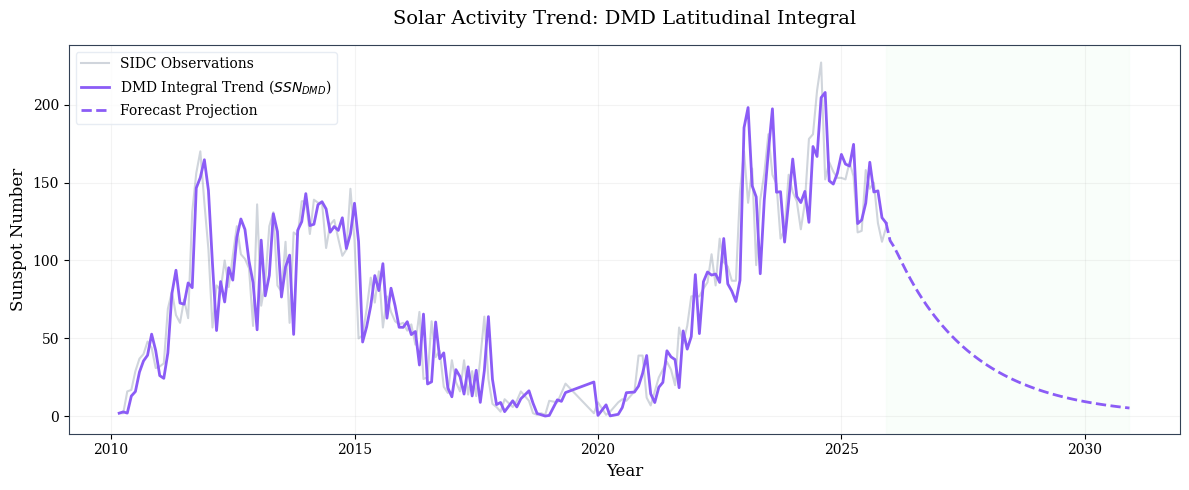
\includegraphics[width=0.92\linewidth]{figures/pred/dmd.png}
    \caption{Número de manchas solares derivado de la integral latitudinal del modelo DMD, $\mathrm{SSN}_{\mathrm{DMD}}(t)$. \textbf{Fuente:} Elaboración propia \citep{schmid2010dmd,kutz2016dmd}.}
    \label{fig:resumen-ssn-dmd}
\end{figure}

\begin{table}[H]
\centering
\caption{Métricas comparativas de validación predictiva para los modelos escalares SSN con ecuaciones de cálculo integradas. \textbf{Fuente:} Elaboración propia con base en los resultados experimentales.}
\label{tab:resumen-prediccion-escalar}
%\scriptsize
\begin{tabular}{lcc}
\toprule
\textbf{Métrica y Ecuación} & \textbf{$\text{SSN}_{\text{PVLK}}$} & \textbf{$\text{SSN}_{\text{DMD}}$} \\
\midrule
$\textstyle \mathrm{MAE}=\frac{1}{N}\sum_{k=1}^{N}|z_k-\widehat{s}_k|$ & 15.31 & 15.22 \\
\addlinespace
$\textstyle \mathrm{RMSE}=\sqrt{\frac{1}{N}\sum_{k=1}^{N}(z_k-\widehat{s}_k)^2}$ & 22.02 & 20.30 \\
\addlinespace
$\textstyle \mathrm{MAPE}=\frac{100}{N}\sum_{k=1}^{N}\left|\frac{z_k-\widehat{s}_k}{z_k}\right|$ & 33.27\% & 32.54\% \\
\addlinespace
$\textstyle R^2=1-\frac{\sum_{k=1}^{N}\left(z_k-\widehat{s}_k\right)^2}{\sum_{k=1}^{N}\left(z_k-\bar{z}\right)^2}$ & 0.8173 & 0.8449 \\
\bottomrule
\end{tabular}
\end{table}

\begin{table}[H]
\centering
\caption{Métricas de validación predictiva espacio-temporal para el modelo DMD-Spörer (Vectorial) con ecuaciones de cálculo integradas. \textbf{Fuente:} Elaboración propia con base en los resultados experimentales.}
\label{tab:resumen-prediccion-vectorial}
%\scriptsize
\begin{tabular}{lc}
\toprule
\textbf{Métrica y Ecuación} & \textbf{Valor} \\
\midrule
$\textstyle E_F=\frac{\|\mathbf{X}-\widehat{\mathbf{X}}\|_F}{\|\mathbf{X}\|_F}$ & 0.4087 \\
\addlinespace
$\textstyle \rho_{ST}=\mathrm{corr}\left(\mathrm{vec}(\mathbf{X}),\mathrm{vec}(\widehat{\mathbf{X}})\right)$ & 0.9126 \\
\addlinespace
$\textstyle \mathrm{MLCE}=\frac{1}{N}\sum_{k=1}^{N}|\theta_{c,k}-\widehat{\theta}_{c,k}|$ & 1.25$^\circ$ \\
\bottomrule
\end{tabular}
\end{table}

El modelo PVL--Kalman resulta más adecuado para seguir la amplitud global del ciclo solar, mientras que DMD aporta una salida no disponible en modelos unidimensionales: la distribución latitudinal y su migración hacia el ecuador. Por ello, ambos modelos se consideran complementarios dentro de la plataforma: uno sintetiza la evolución temporal del SSN y el otro conserva estructura espacial útil para interpretación científica \citep{hathaway2015solarcycle,podladchikova2012kalman,kutz2016dmd}.

\subsection{Validación integral del sistema}

La validación del hardware documentó el montaje de la cámara, la atenuación solar, la unidad de preprocesamiento y la integración con el telescopio. Además, una captura real realizada el 2026-05-05 permitió verificar adquisición, guardado local, preprocesamiento y sincronización con la base de datos bajo condiciones de operación de campo \citep{zwoASILinuxManual,raspberryPi5Docs2026}.

\begin{table}[H]
\centering
\caption{Métricas operativas representativas de la Raspberry Pi 5 durante la validación. \textbf{Fuente:} Elaboración propia.}
\label{tab:resumen-raspberry-operacion}
%\scriptsize
\begin{tabular}{lc}
\toprule
\textbf{Métrica} & \textbf{Valor representativo} \\
\midrule
Captura de imagen individual & 420 ms \\
Guardado local en microSD & 180 ms \\
Preprocesamiento básico por imagen & 1350 ms \\
Sincronización a Supabase & 3800 ms/imagen \\
Uso medio de CPU & 38\% \\
Uso máximo de CPU & 72\% \\
Uso de RAM del servicio local & 3.3 GB \\
Temperatura tras 25 min & 57 $^{\circ}$C \\
\bottomrule
\end{tabular}
\end{table}

Durante las pruebas no se observaron reinicios, cierres del servicio ni reducción térmica perceptible bajo refrigeración activa. Estos resultados respaldan la viabilidad del prototipo como nodo local de captura y asistencia, siempre que se mantenga ventilación adecuada y se considere la variabilidad de red durante la sincronización \citep{raspberryPi5Docs2026,nmcliHotspot2026}.

\begin{figure}[H]
    \centering
    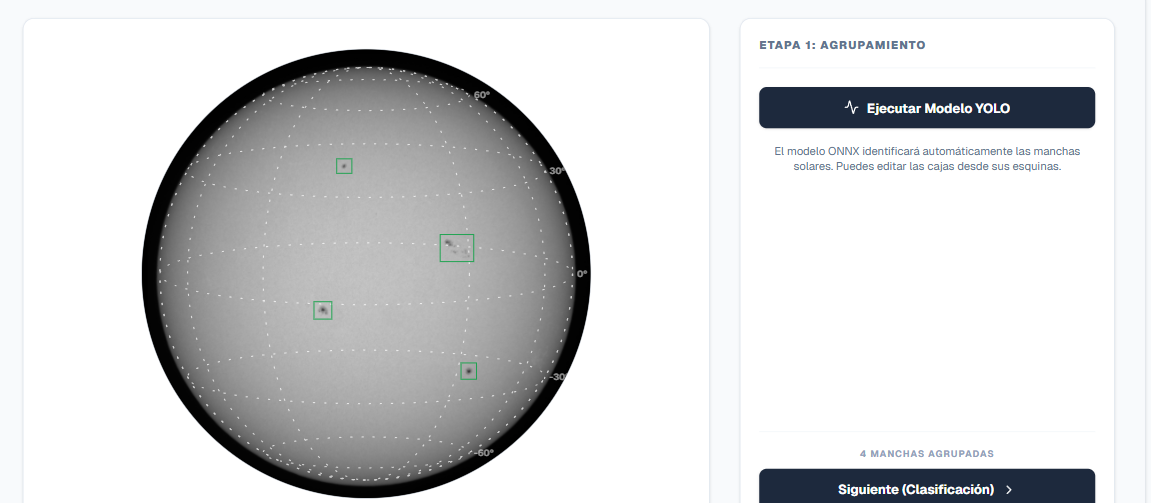
\includegraphics[width=0.9\linewidth]{figures/web/yolo.png}
    \caption{Validación de la etapa de agrupamiento \textit{on-device} mediante YOLO en la plataforma web. \textbf{Fuente:} Elaboración propia.}
    \label{fig:resumen-web-yolo-validacion}
\end{figure}

\begin{figure}[H]
    \centering
    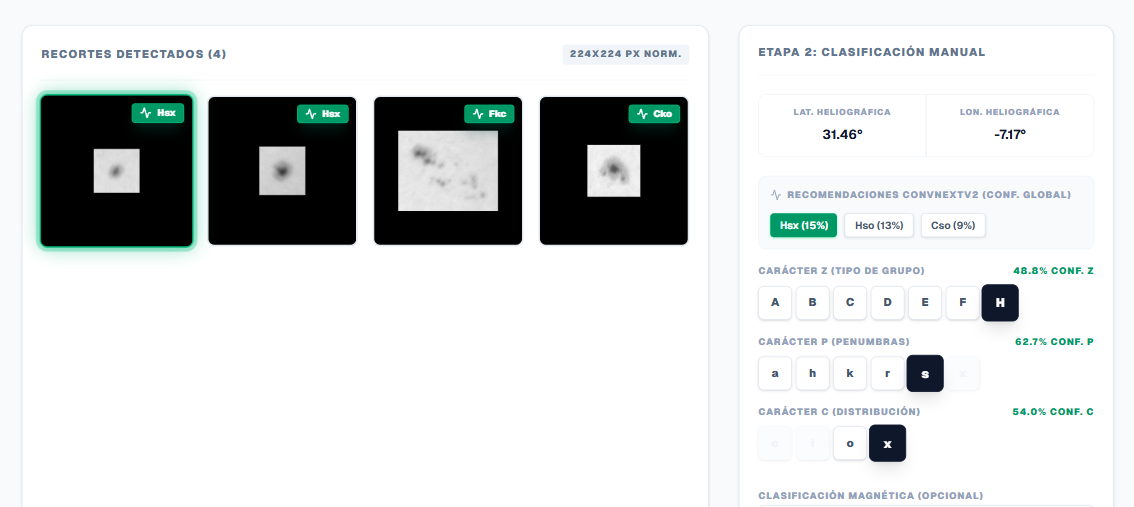
\includegraphics[width=0.9\linewidth]{figures/web/convnext.png}
    \caption{Validación de la etapa de clasificación morfológica \textit{on-device} mediante ConvNeXtV2 en la plataforma web. \textbf{Fuente:} Elaboración propia.}
    \label{fig:resumen-web-convnext-validacion}
\end{figure}

La plataforma web se validó mediante carga de modelos, consulta de datos desde Supabase e inferencia local en navegador; las Figuras~\ref{fig:resumen-web-yolo-validacion} y~\ref{fig:resumen-web-convnext-validacion} documentan, respectivamente, el agrupamiento con YOLO26n y la clasificación morfológica con ConvNeXtV2a. La ejecución se configuró con WebAssembly para aproximar el comportamiento en dispositivos sin aceleración GPU dedicada, verificando que los modelos ONNX pueden descargarse y ejecutarse como parte del flujo de asistencia observacional \citep{camporeale2019ml,ultralyticsYOLO26,woo2023convnextv2}.

\begin{table}[H]
\centering
\caption{Rendimiento resumido de la plataforma web durante la validación. \textbf{Fuente:} Elaboración propia.}
\label{tab:resumen-web-rendimiento}
%\scriptsize
\begin{tabular}{lc}
\toprule
\textbf{Métrica} & \textbf{Valor} \\
\midrule
Proveedor de ejecución & WASM \\
Tiempo de descarga del modelo & 5803 ms \\
Tiempo de galería Supabase & 1702 ms \\
Inferencia YOLO & 3105 ms \\
Inferencia de clasificación & 3201 ms \\
\bottomrule
\end{tabular}
\end{table}
